\chapter{Metodologie per la classificazione}
\label{metodologie}

\section{Feature hand-crafted}
% \cite{spathis2016photo}
Dopo aver suddiviso le immagini del dataset GPD come già illustrato nel Capitolo~\ref{GPD} sono stati osservati i vari tipi di feature in letteratura, al fine di capire quali utilizzare. Le feature possono essere suddivise in 4 principali categorie \cite{spathis2016photo}:
\begin{enumerate}
\item \textbf{Feature relative al colore}, ad esempio combinazioni lineari dei tre canali degli spazi colore HSV o HSL oppure la media di essi. 
\item \textbf{Feature relative alla texture}, ad esempio lo studio degli edge, LBP (Local Binary Pattern), CEDD (Color and Edge Directivity Descriptor) o QHist ovvero l'istogramma dei canali RGB quantizzati a 16 livelli ciascuno.
\item \textbf{Feature relative alla composizione}, ad esempio lo studio del blur, delle linee tramite la trasformata di Hough, l'aspect ratio o la regola dei terzi.
\item \textbf{Feature relative al contenuto}, ovvero la ricerca di determinati oggetti o aree in una immagine, ad esempio un volto oppure la pelle.
\end{enumerate} 

\section{Un'ulteriore suddivisione delle immagini}
\label{divisione}
Dopo aver analizzato più a fondo i datastore, ovvero le strutture utilizzate in MATLAB \cite{MATLAB} per gestire i vari set di immagini, è stato scelto di lavorare con set bilanciati in modo da avere una probabilità equa per le due classi. 

In particolare le immagini sono state ulteriormente divise come segue:
\begin{itemize}
  \item \textbf{Set di Rigetto}: 2176 immagini positive che portavano le due classi ad essere sbilanciate, in particolare questo set di immagini non verrà più utilizzato nel proseguo del lavoro. Si avranno 21824 immagini in totale, ovvero la differenza tra il numero totale di immagini (24000) e il numero di immagini appartenenti a questo set.
\item \textbf{Training set}: 17678 immagini, ovvero il 90\% del 90\% del nuovo numero totale di immagini (21824). Si prende una prima volta il 90\% delle immagini poiché il restante 10\% sarà poi parte del Test set, successivamente se ne prende ancora il 90\% perché il restante 10\% sarà assegnato al Validation set. In particole le immagini del Training set saranno divise come segue:
  \begin{itemize}
  \item 8839 positive
  \item 8839 negative
  \end{itemize}
  \item \textbf{Test set}: 2182 immagini, ovvero il restante 10\% dopo la prima divisione, di cui
  \begin{itemize}
  \item 1091 positive
  \item 1091 negative
  \end{itemize}
  \item \textbf{Validation set}: 1964 immagini, ovvero il restante 10\% dopo la seconda divisione del Training set, di cui
  \begin{itemize}
  \item 982 positive
  \item 982 negative
  \end{itemize}
\end{itemize}

\section{Feature estratte da una rete neurale}

Per cercare di migliorare i risultati ottenuti con le feature hand-crafted si è scelto di utilizzare una rete neurale da cui estrarre delle feature di più alto livello e passarle a un classificatore, in questo caso un SVM. La rete scelta per questa fase è stata la ResNet-18 poiché era quella più utilizzata in altri esperimenti \cite{sheng2021learning} presi come riferimento e che allo stesso tempo otteneva anche buoni risultati.
% eventualmente grafico resnet18

È stato ipotizzato anche l'uso della VGG-16 ma è stata preferita la ResNet-18 in quanto dopo alcuni test si è notato che era più lenta nel riaddestramento e anche meno utilizzata negli esperimenti presi come riferimento.

Quando bisogna estrarre le feature da una rete neurale è necessario specificare il layer della rete da cui estrarle, in questo caso con la rete ResNet-18 sono stati fatti due test, uno con il layer pool5 e uno con il layer res3b\_relu. Essi si trovano in parti diverse della rete, infatti il layer pool5 si trova alla fine della rete, mentre il layer res3b\_relu si trova più o meno a metà di essa.


\section{Uso di una rete neurale per l'intera classificazione}

\subsection{Prima implementazione}
Al fine di incrementare ulteriormente l'accuratezza ottenuta nelle fasi precedenti del lavoro si è scelto di utilizzare una ResNet-18 pre-addestrata su cui svolgere una operazione di Fine Tuning, ovvero una parziale modifica della rete al fine di adattarla per svolgere un nuovo task. In particolare in questa fase sono stati modificati il Fully Connected layer e il Classification Output layer in modo tale che lavorino con due classi e restituiscano in output solo una di esse. 

Nella fase di riaddestramento della rete è stato necessario scegliere se compiere delle operazioni di aumento del dataset disponibile in particolare, traendo ispirazione dal lavoro originale \cite{sheng2021learning}, si è scelto di compiere scaling sia lungo l'asse x che lungo l'asse y, traslazione e riflessione rispetto all'asse x in maniera casuale al fine di aumentare il numero di immagini disponibili. 

É stato necessario anche impostare alcuni parametri tra cui il numero massimo di epoche, ovvero il massimo numero di cicli di training, la dimensione del batch, ovvero un parametro che definisce il numero di campioni con cui lavorare prima di aggiornare i parametri interni al modello, e il tasso di apprendimento iniziale della rete neurale.


\subsection{Early Stopping}

Durante la fase di riaddestramento della rete si è osservato che, dopo un determinato periodo di tempo, il grafico dell'accuratezza tendeva a rimanere costante e ciò significa che la rete non stava più apprendendo nulla dai dati forniti ad essa. Per questo motivo si è scelto di implementare l'Early Stopping o stop anticipato, il quale permette di fermare il processo di training se l'accuratezza non migliora oppure se la funzione Loss peggiora per un certo numero di epoche consecutive. 

In questo caso si è scelto di implementare lo stop basandosi sull'accuratezza, ad esempio se si sceglie di fermare l'addestramento dopo due epoche dove l'accuratezza non si incrementa di fatto si otterranno almeno tre epoche di training, in quanto la rete controllerà se l'accuratezza si è mantenuta minore o uguale a quella della prima epoca nelle due epoche successive e, in caso affermativo, fermerà il processo.

Lo stop anticipato può permettere un risparmio di tempo e risorse durante il Fine Tuning, ma ciò dipende da come si impostano i parametri iniziali e dal numero di epoche dopo le quali si sceglie di fermare il processo. 

É importante segnalare che il processo di Early Stopping potrebbe non essere sempre vantaggioso in quanto è possibile ottenere anche casistiche nelle quali, nonostante lo si utilizzi, vengano comunque compiute tutte le epoche di training perché l'accuratezza risulterà sempre in crescita e quindi la rete non fermerà il training in anticipo, poiché si cerca sempre di ottenere il miglior risultato possibile.
 
% TO DO: Nel Capitolo dei Risultati va inserita una sezione per riportare l'accuratezza ottenuta sul mio Dataset, con eventuali problematiche legate agli exif
 
\section{Valutazione del dataset proposto}
\label{valutazione}
Per tutto il resto del lavoro è stata utilizzata la rete ResNet-18 riaddestrata con Early Stopping che ha ottenuto migliori risultati sia sul test set che sul validation set, ovvero quella con Initial Learn Rate pari a 0.0005, stop anticipato dopo due epoche delle sei epoche possibili e dimensione del batch pari a dieci.

Con questa rete sono state valutate le immagini del dataset proposto, prestando attenzione al fatto che in MATLAB alcune immagini erano visualizzate ruotate di 90 gradi a causa di metadati contenuti all'interno delle immagini stesse, per cui è stato necessario un processing mirato su alcune immagini al fine di avere tutto il dataset visualizzato correttamente. 

Inizialmente, come già specificato, si era pensato di utilizzare come groundtruth delle label ricavate secondo il criterio che una fotografia professionale fosse esteticamente bella, e quindi avesse label positiva, mentre una fotografia scattata da un utente non lo fosse, e quindi avesse label negativa. Ciò è parso poco sensato, in quanto osservando le immagini del dataset proposto riportate nel Capitolo~\ref{new_dataset} in Figura \ref{negativeNew} e Figura \ref{positiveNew} si può notare che alcune immagini non professionali sono state comunque etichettate come positive dagli utenti nel questionario a loro sottoposto e viceversa, ciò sta a significare che non sempre c'è una corrispondenza tra tecnica nello scatto ed estetica di esso, anche se generalmente molte fotografie professionali sono percepite come esteticamente belle poiché utilizzano colori, contrasti e tecniche che gli utenti apprezzano molto.

A seguito di questa considerazione si è quindi scelto di utilizzare come groundtruth per la valutazione le label risultanti dal questionario, in quanto esse catturano in maniera particolare la percezione dell'estetica del dataset proposto da parte di un particolare gruppo di 41 utenti che sono stati presi come campione per questo esperimento. In particolare le immagini saranno distribuite nelle due classi come segue:
\begin{itemize}
\item \textbf{Groundtruth appartenente alla classe positiva}: 73 immagini
\item \textbf{Groundtruth appartenente alla classe negativa}: 27 immagini
\end{itemize}


\section{Grad-CAM per capire le predizioni}

Al fine di comprendere quali porzioni di un'immagine vengano maggiormente prese in considerazione dalla rete per determinare la label predetta è stata utilizzata la tecnica del Gradient-weighted Class Activation Mapping (Grad-CAM) \cite{selvaraju2017grad}, la quale evidenzia in rosso le aree più significative e in blu quelle meno significative per la predizione della rete fornendo una visualizzazione facilmente interpretabile da chi la osserva ed essendo applicabile a molte famiglie di reti neurali convoluzionali. 

In particolare la tecnica in questione utilizza il gradiente relativo al concetto che si è scelto come target nell'immagine, il quale entra negli ultimi layer convoluzionali, con l'obiettivo di produrre una mappa che mostri le aree più significative e quelle meno significative relative al tema scelto. Si utilizzano proprio questi layer poiché le feature convoluzionali conservano informazioni spaziali, le quali vengono perse all'interno del Fully Connected layer e quindi gli ultimi layer convoluzionali prima di esso permettono di conciliare una buona semantica con queste informazioni che sono molto significative se, come in questo caso, si vuole analizzare quale area dell'immagine è più rilevante per la classificazione di essa da parte di una rete neurale.

Un esempio di applicazione della tecnica Grad-CAM ad una immagine è riportato in Figura \ref{gradcam_gen}.

\begin{figure}[H]
\centering
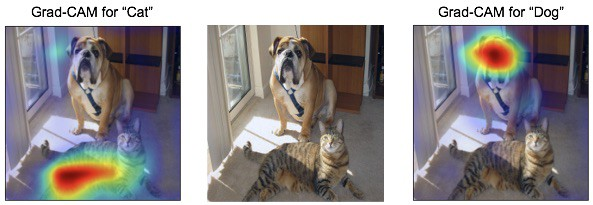
\includegraphics[height=50mm]{images/gradcam_generica.jpg}
\caption{Esempio di una immagine a cui è stata applicata la tecnica Grad-CAM focalizzandosi su due differenti classi di oggetti, in questo caso prima sulla classe "Gatto" e poi sulla classe "Cane", il quale è stato tratto dal lavoro originale sulla tecnica Grad-CAM \cite{selvaraju2017grad}}
\label{gradcam_gen}
\end{figure}

%%%%%
\begin{comment}
\begin{figure}[H]
\centering
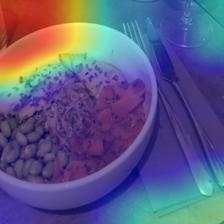
\includegraphics[height=45mm]{images/gradcam1.jpg}
\quad
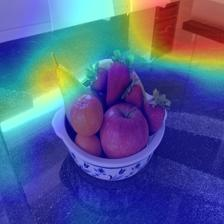
\includegraphics[height=45mm]{images/gradcam23.jpg}
\quad
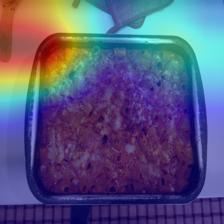
\includegraphics[height=45mm]{images/gradcam14.jpg}
\quad
\caption{Esempi di immagini a cui è stata applicata la tecnica Grad-CAM dove la rete ha predetto correttamente una label negativa}
\label{gradcam_neg}
\end{figure}

\begin{figure}[H]
\centering
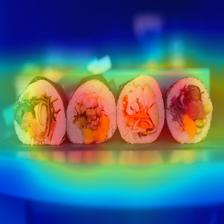
\includegraphics[height=45mm]{images/gradcam53.jpg}
\quad
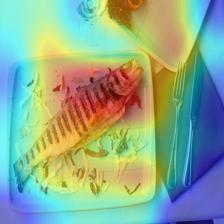
\includegraphics[height=45mm]{images/gradcam85.jpg}
\quad
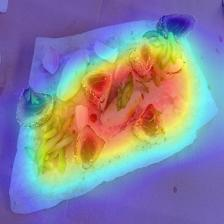
\includegraphics[height=45mm]{images/gradcam28.jpg}
\quad
\caption{Esempi di immagini a cui è stata applicata la tecnica Grad-CAM dove la rete ha predetto correttamente una label positiva}
\label{gradcam_pos}
\end{figure}
\end{comment}
%%%%%

Osservando le immagini ricavate con la tecnica appena illustrata applicata alle immagini del dataset proposto sembrava potesse esserci una correlazione tra la predizione della rete e la porzione di immagine che veniva considerata più significativa, ovvero quella colorata di rosso.

Al fine di avere una misura oggettiva che potesse aiutare a comprendere se ci fosse o meno questa correlazione è stato necessario compiere alcuni passaggi preliminari:

\begin{itemize}
\item \textbf{Creazione di maschere binarie}, le quali avessero in bianco il cibo e in nero il background, un esempio è riportato in Figura \ref{mask}. Esse sono state realizzate con l'ausilio di Photoshop, ma sarebbe andato bene anche un altro editor di immagini.
\begin{figure}[H]
\centering
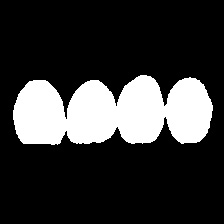
\includegraphics[height=45mm]{images/Resized53.jpg}
\quad
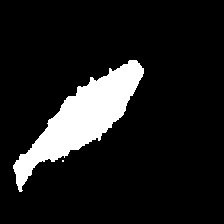
\includegraphics[height=45mm]{images/Resized85.jpg}
\quad

\includegraphics[height=45mm]{images/Resized1.jpg}
\quad
\caption{Esempi di maschere binarie dei cibi, le quali mostrano in bianco il cibo e in nero il background}
\label{mask}
\end{figure}
\item \textbf{Calcolo del rapporto tra area della maschera e area totale dell'immagine}, tale rapporto è stato espresso in percentuale ed è indicato con $A_{m}$.
\item \textbf{Calcolo del rapporto tra energia che ricade nella maschera ed energia totale}, dove con energia si intende l'intensità della mappa Grad-CAM per ogni pixel. Questo passaggio è stato fatto ponendo attenzione a normalizzare i valori delle mappe Grad-CAM rispetto al valore minimo e massimo, in modo tale da ottenere valori tra zero e uno, come segue:
\begin{equation} 
\label{normalizzazione_minmax}
x^{'}=\frac{x-min}{max-min}
\end{equation}
In particolare anche questo rapporto è stato espresso in percentuale per comodità e viene indicato con $E_{m}$.
\item \textbf{Calcolo dell'indicatore di concentrazione dell'energia}, ovvero calcolo del seguente rapporto:
\begin{equation} 
\label{indicatore}
C=\frac{E_{m}}{A_{m}}
\end{equation}
Tale valore per definizione sarà un valore decimale e non una percentuale, poiché è definito come rapporto tra due percentuali. Si è scelto di mantenerlo in questa forma per comodità nel visualizzare grafici che lo rappresentassero al fine di correlarlo alle predizioni della rete. 
\end{itemize}